\chapter{Antecedentes}

\section{Historia Clínica}

Actualmente en la mayoría de los centros de salud la información que compone la Historias Clínicas de cada paciente es almacenan mediante documentos físicos, en su mayoría totalmente elaborados a mano, en otros casos usando plantillas con campos preformateados (como se puede observar en las figuras 3.1 y 3.2), lo cual genera varios problemas.\\[0.1cm]

En cuanto los diferentes centros de salud donde se pudo relevar al software existente y su aplicación a la manipulación de historia clínica, este suele ser muy incompleto y abocado a la especialidad del médico, es por ello que si esta informatizado cada área suele manejar sistemas que terminan siendo incompatibles entre sí.\\[0.1cm]

\begin{figure}[h]
    \centering
    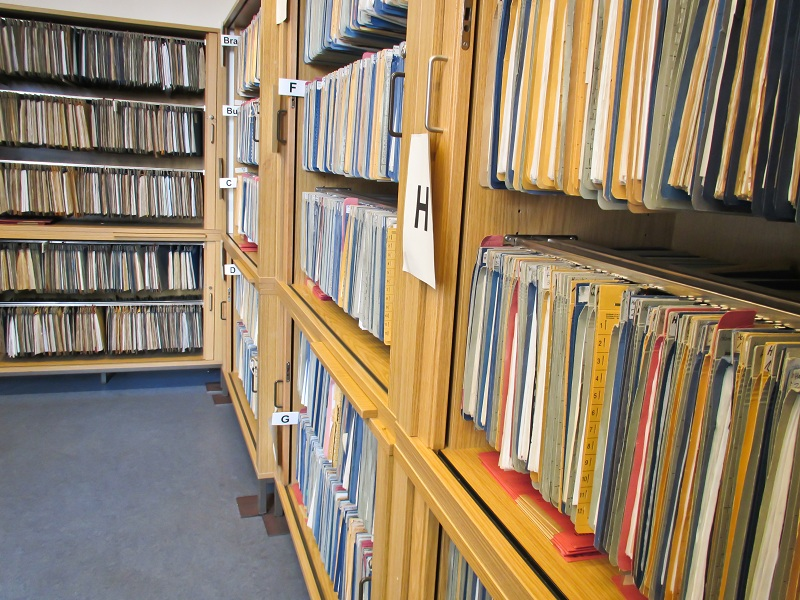
\includegraphics[scale=1.5]{resourse/folders-archivos.jpg}
    \caption{Almacenamiento Físico de Archivos}
    \label{fig:05}
\end{figure}  


\begin{figure}[H]
    \centering
    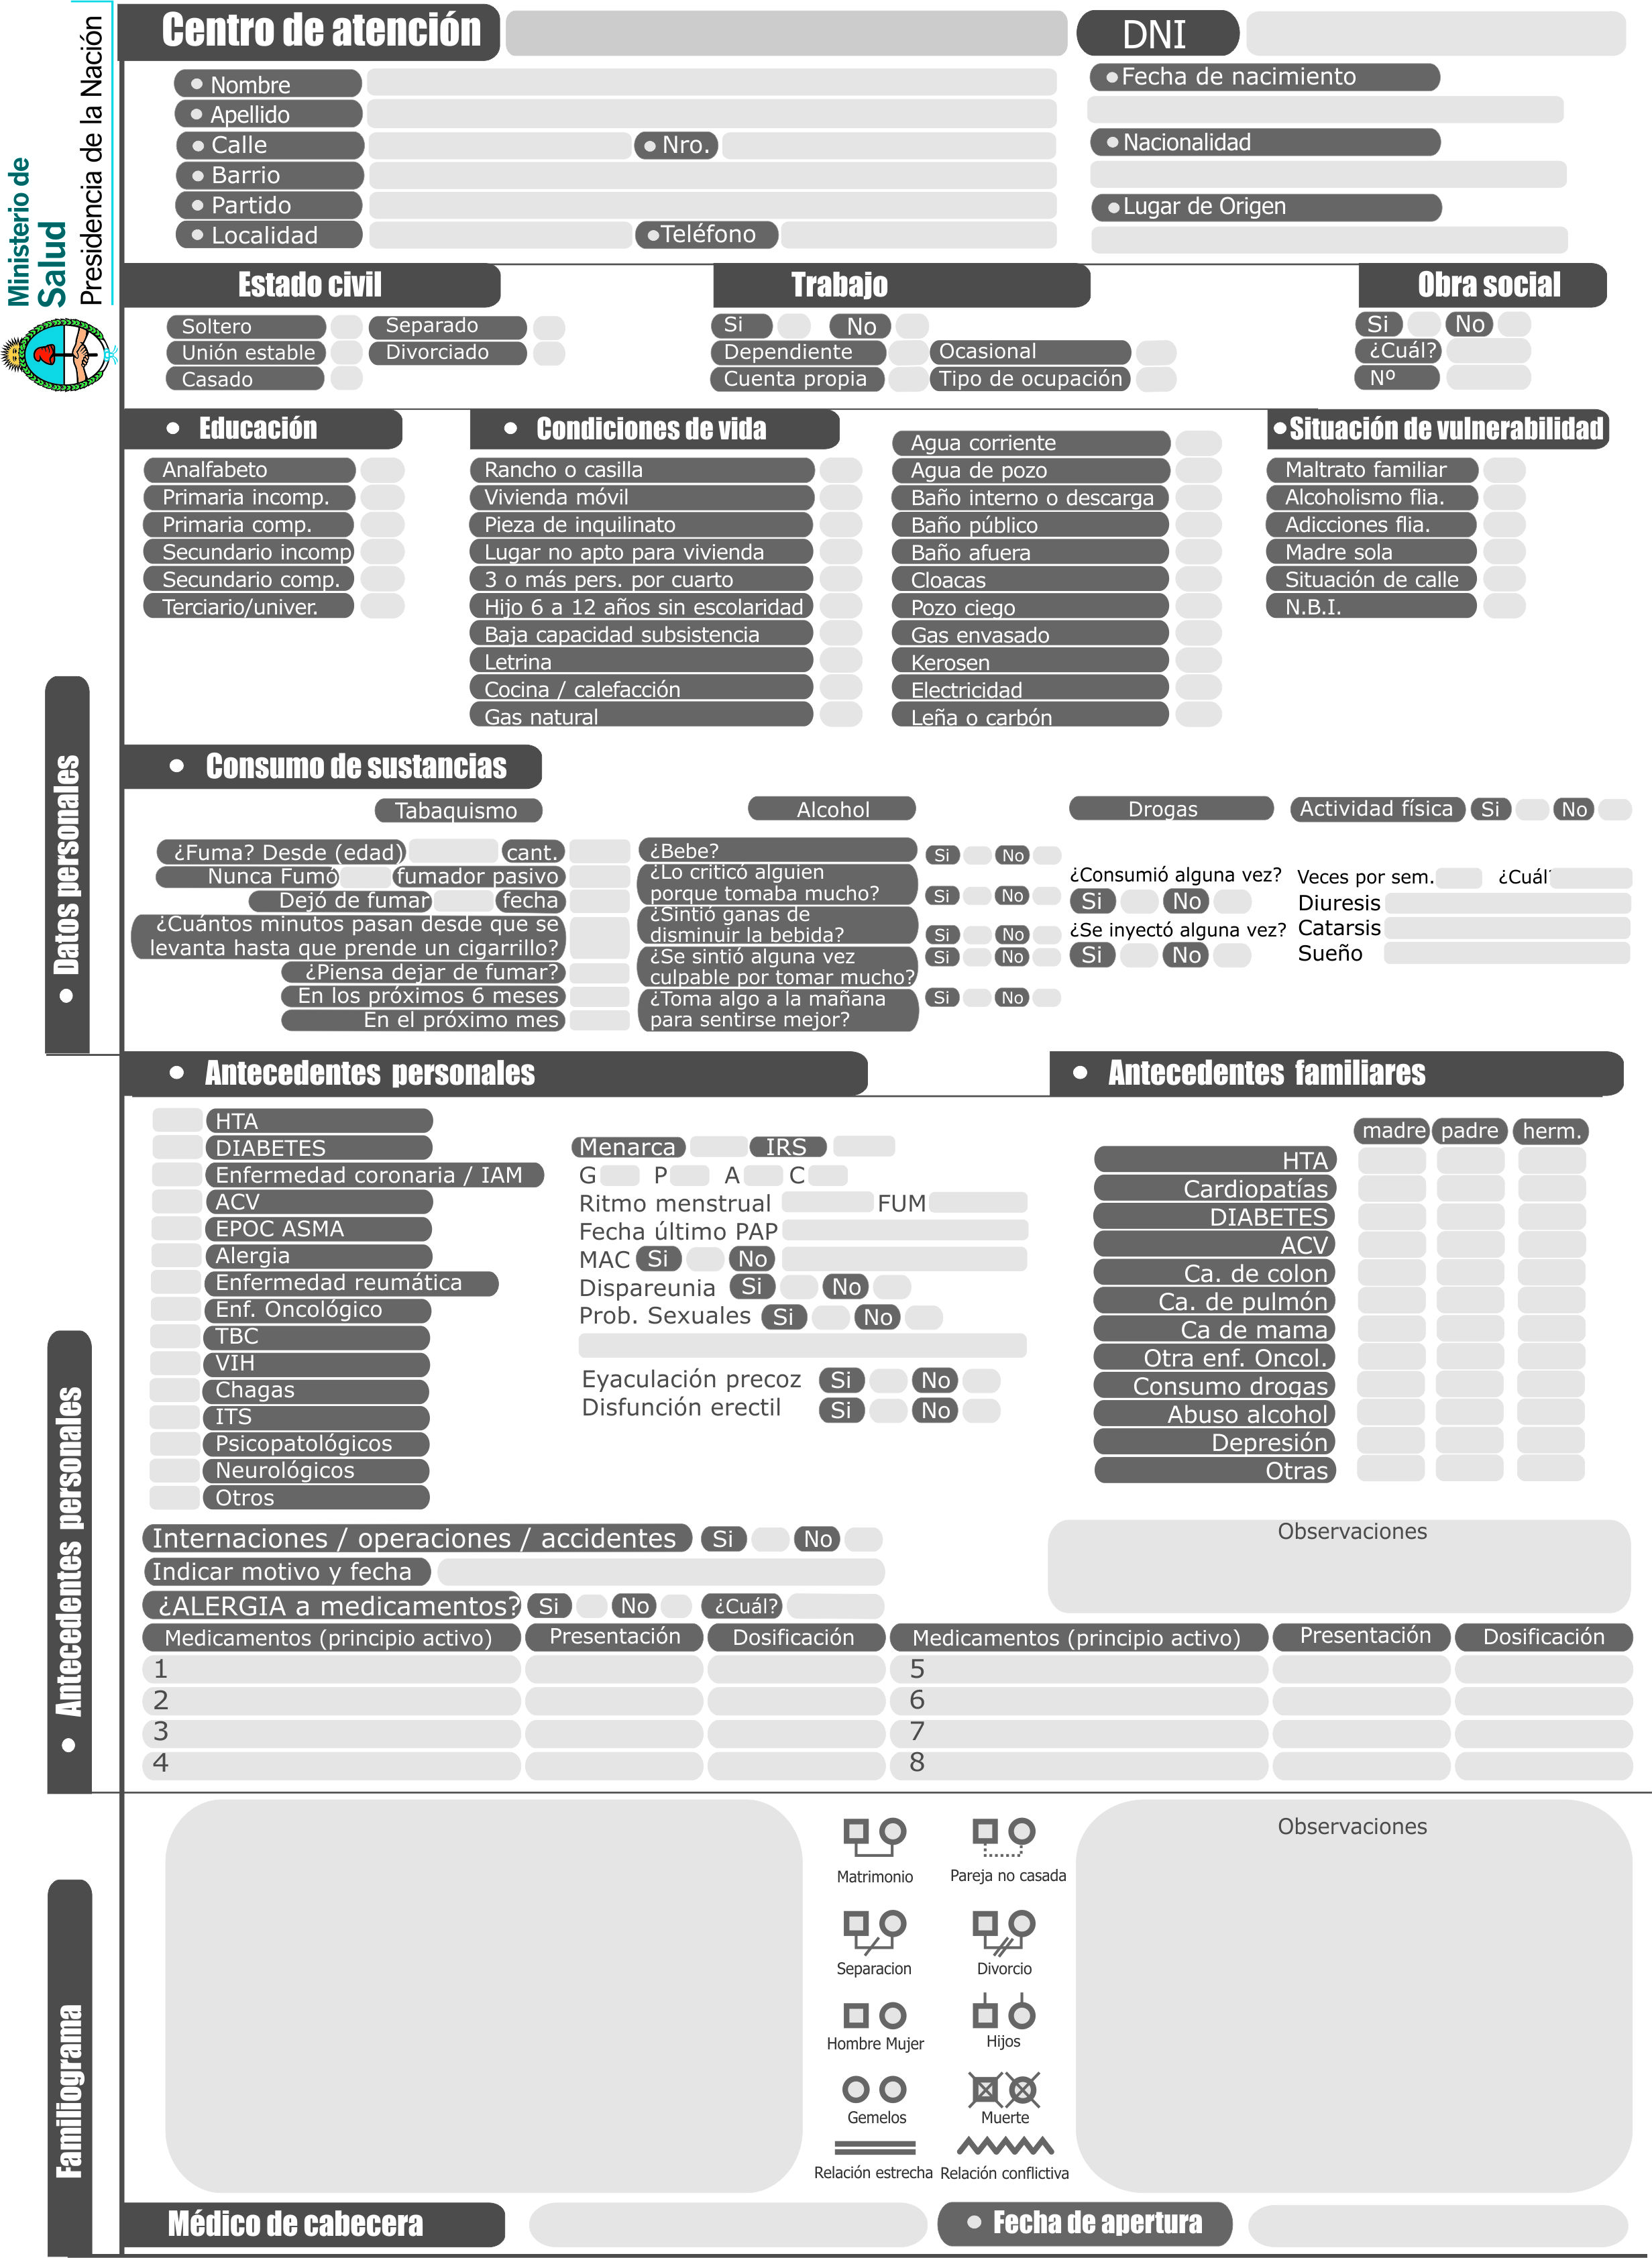
\includegraphics[scale=0.7]{resourse/historia-clinica-f.jpg}
    \caption{Modelo Historia Clínica Ministerio de Salud de La Nación Pag 1}
    \label{fig:06}
\end{figure}  

\begin{figure}[H]
    \centering
    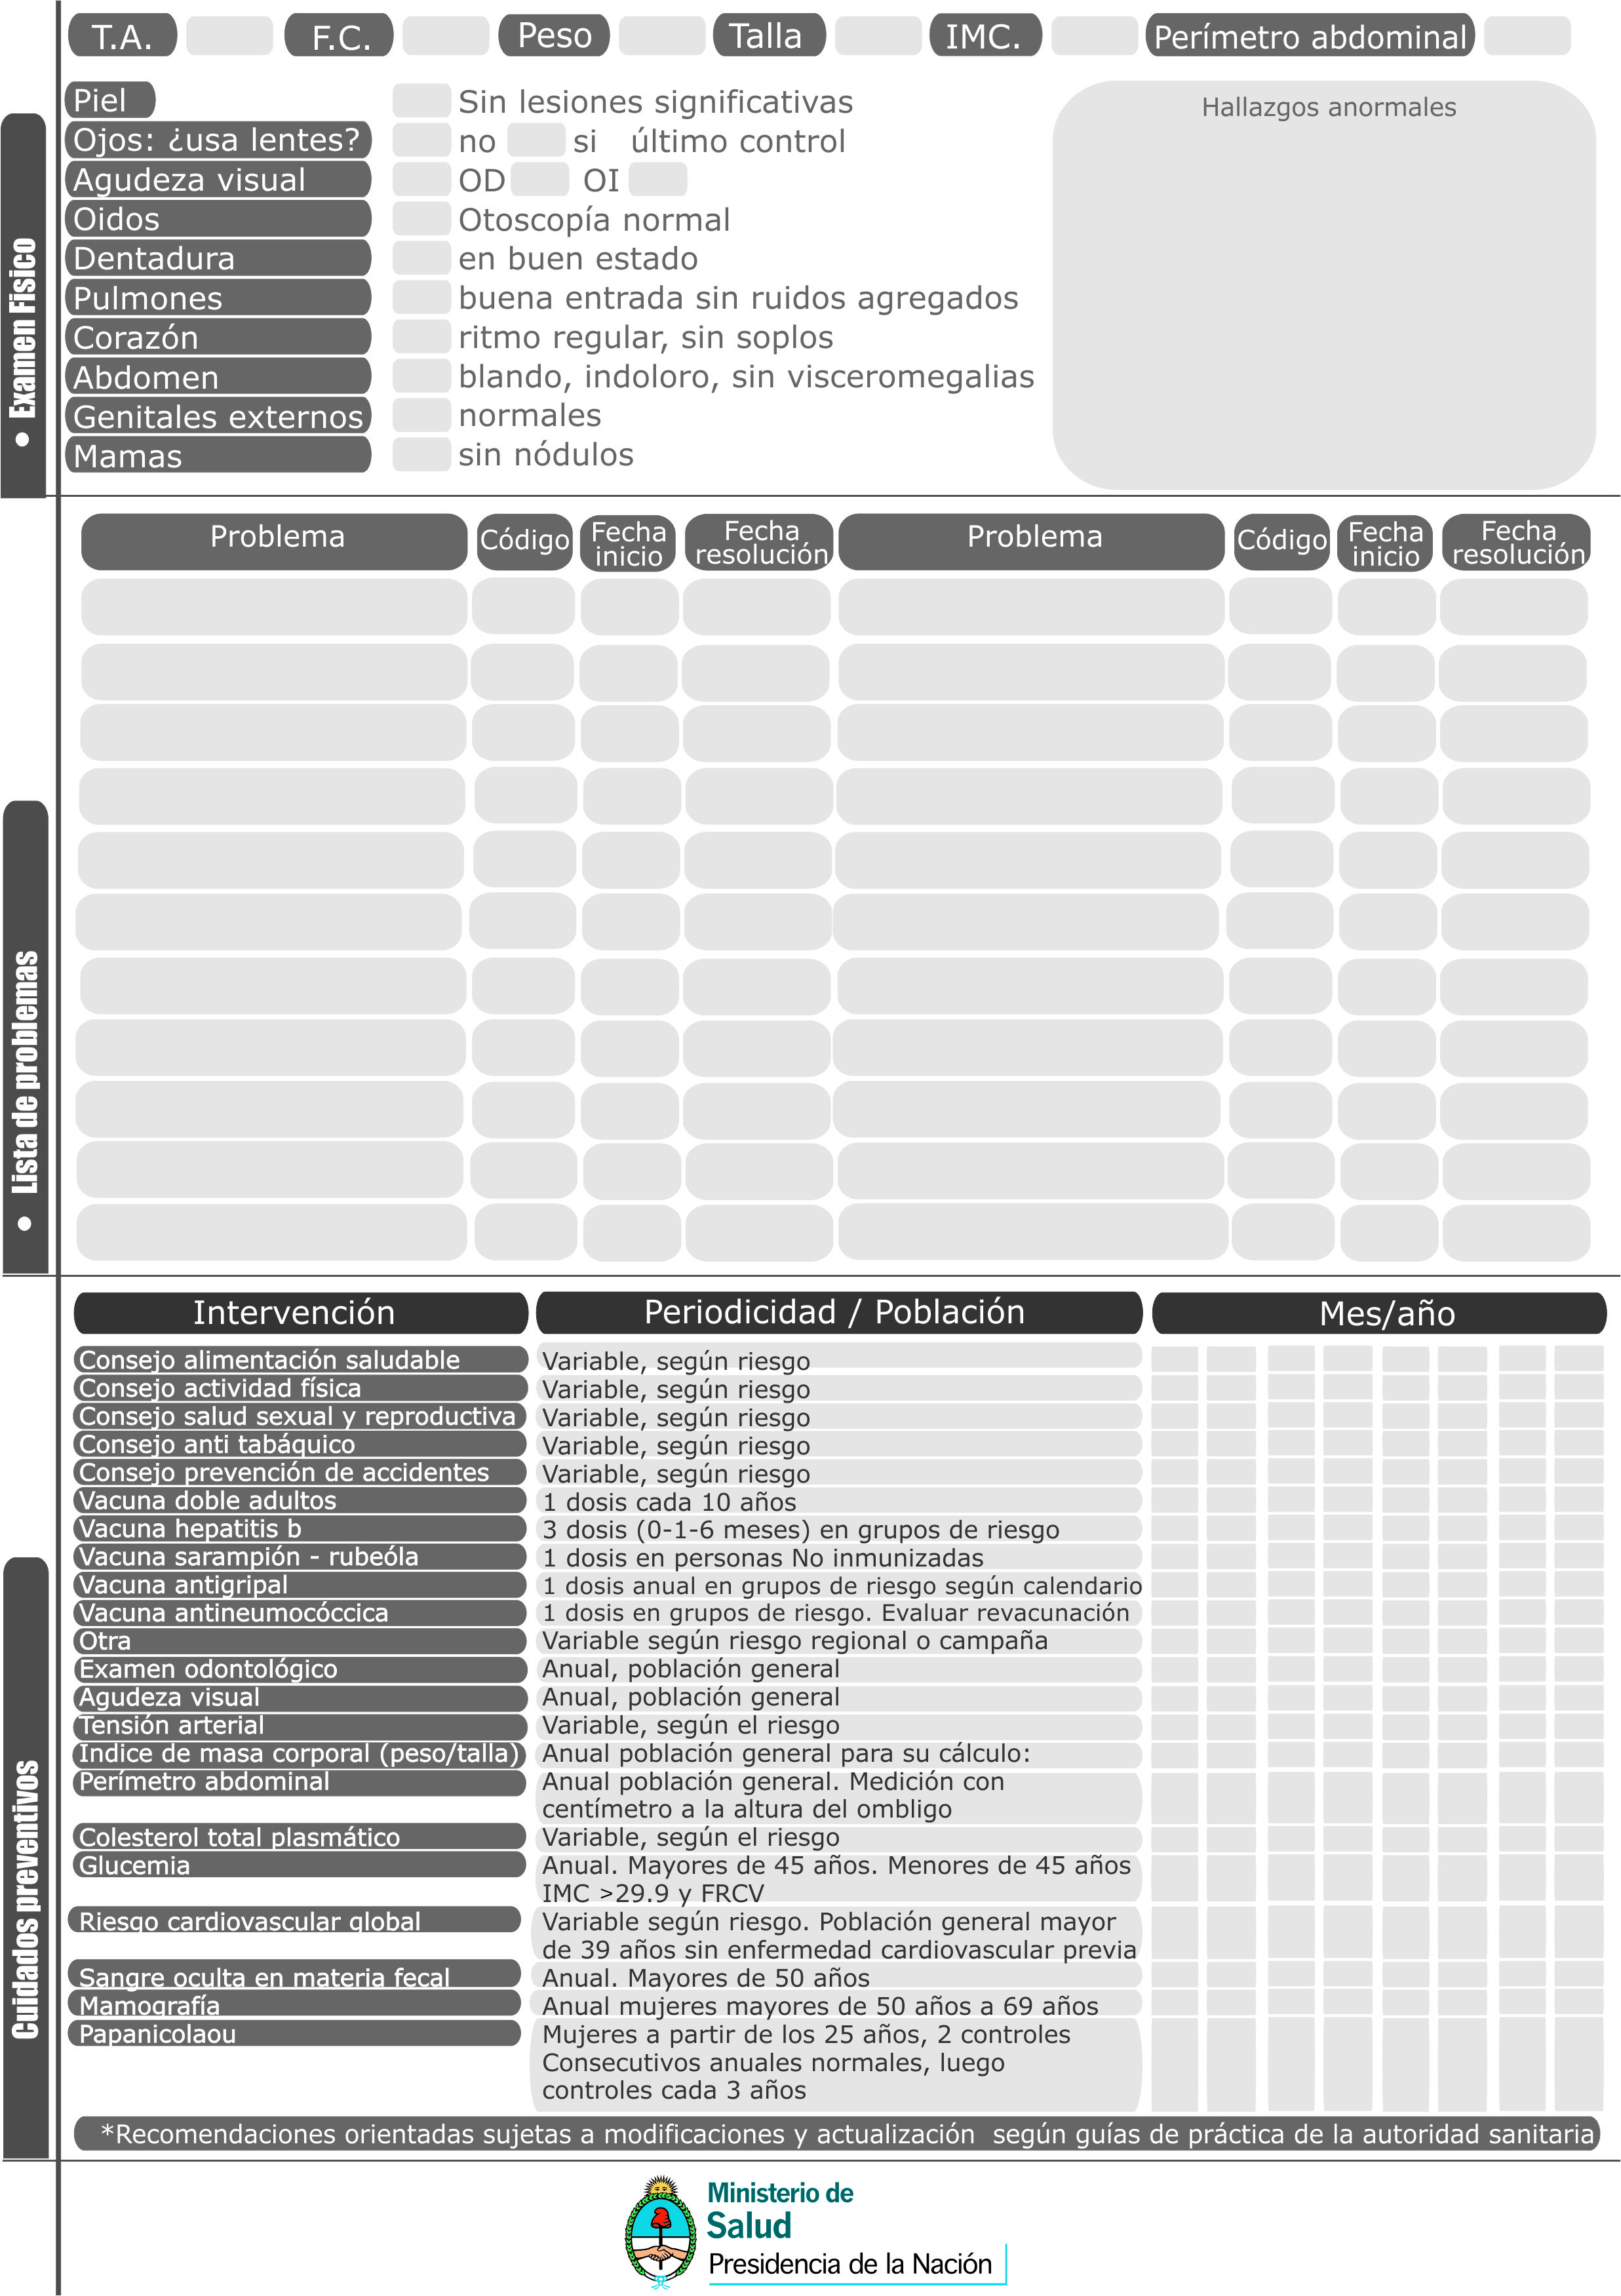
\includegraphics[scale=0.7]{resourse/historia-clinica-d.jpg}
    \caption{Modelo Historia Clínica Ministerio de Salud de La Nación Pag 2}
    \label{fig:07}
\end{figure}

\section{Problemas del Sistema Actual}

Nos referimos al \textit{Sistema Actual} en cuanto a cómo funcionan las organizaciones en nuestro caso consultorios médicos y solo hablamos del software que haya implantado sino al funcionamiento del mismo viendo la organización desde un enfoque sistémico \footnote{Bajo este enfoque el mundo se organiza en torno a sistemas que funcionan y a través de los cuales se ordena la sociedad. El elemento central del enfoque sistémico es la estructura, que permanece estable a pesar de los cambios sociales que se produzcan. Se puede consultar más acerca del Enfoque Sistémico o la TGS en \cite{EnfSys}.}. Paso a describir algunos de los problemas a los que se enfrentan las organizaciones cuando almacenan las historias clínicas en formato papel:

\subsection{Almacenamiento}
 A medida que crece el número pacientes y la información que va anexando a cada Archivo se va necesitando más espacio físico para almacenar dicha información. Por ello con el paso del tiempo las instalaciones dedicadas a tal fin suelen verse colapsadas por los grandes volúmenes de información que deben manejar.\\[0.1cm]

\subsection{Búsqueda y Localización}
La Búsqueda de expedientes se puede agilizar un poco utilizando una buena organización, el problema es que la mayoría de los edificios para tal fin, suelen estar saturados por grandes volúmenes de archivos físicos, Por lo que encontrar un archivo requerido suele ser una tarea costosa y lenta.\\[0.1cm]

\subsection{Deterioro}
En lo que hace a la conservación propiamente dicha, el combate de los problemas habituales que se derivan de las condiciones climáticas, de la humedad, de las plagas, del deterioro natural del papel, especialmente por su fabricación con celulosa desde hace dos siglos, es una constante que, pese a sus avances, no ha encontrado soluciones definitivas. Por ende, una preocupación común a los archivos y bibliotecas, es encontrar remedios prácticos y asequibles para asegurar la preservación de sus acervos. De lo anterior se desprende la necesidad, en el nivel nacional, de procurar el establecimiento de políticas y normas sobre conservación en las instituciones públicas y privadas dedicadas a la protección del patrimonio.\\[0.1cm]

\subsection{Otros Problemas}
Otros problemas que acarrean el uso de archivos físicos son:

\begin{itemize}
    \item Perdida, alteración o dato de documentos importantes
    \item Gasto excesivo en fotocopias
    \item Altos costos de personal para administrar, suplir, mantener y recuperar el archivo físico
    \item Costos asociados al transporte de documentos ya sea interna o externamente
    \item Costos asociados al espacio físico requerido para su almacenamiento
    \item Falta de condiciones adecuadas para el almacenamiento de documentos como: ventilación, humedad, temperatura
    \item Falta de respaldo adecuado en caso de catástrofe como incendio, inundación o terremoto
\end{itemize}


\subsection{La Solución Planteada}

Por ello este era un escenario perfecto donde es necesario informatizar el actual sistema, lo cual solucionaría los 2 principales problemas del mismo que son el Excesivo espacio de almacenamiento y el lento trabajo de búsqueda además de:

\begin{itemize}
    \item Reducir costos de personal administrativo, ya que las búsquedas y registro las hará el sistema.
    \item Brindar la información de manera rápida en situaciones críticas que requieren un rápido accionar por parte del médico.
   \item Disponibilidad en todo momento y cualquier lugar para consulta por parte de los médicos ya que solo requerirá disponer de un usuario y un ordenador con conexión a Internet para poder consultar.
\end{itemize}

Es cierto que los sistemas informáticos sufren problemas de almacenamiento, búsqueda (en el caso de grandes volúmenes de información) y deterioro por el paso del tiempo pero en este caso el primero se soluciona agregando más espacio de disco, cosa que hoy en día es algo relativamente barato a razón de 1 peso = 1 Gb. \footnote{Gb hace referencia a Gigabyte que es una medida utilizada en informática la cual normalmente hace referencia a tamaños de almacenamiento.}.  \\[0.1cm]

El problema de las búsqueda no afecta mucho con la velocidad de los equipos actuales se puede consultar bases de datos con millones de registro en unas pocas milésimas de segundos dicho tiempo resulta imperceptible para la persona en la mayoría de las veces, en todo caso dependerá de la implementación y el motor de bases de datos más que de las prestaciones del hardware.\\[0.1cm]

En cuanto al deterioro, puede que con el tiempo los equipos de hardware tales como discos duros fallen en algún momento, pero esto es salvable siempre y cuando se realicen buenas prácticas tales como implementar un sistemas de backup, también replicación de datos en caso de que se necesite alta disponibilidad de la información que se almacena.\\[0.1cm]


\section{Gestión de Turnos}   

En lo que respecta a asignación de turnos, el sistema actual en la mayoría de los casos no ha tenido un mejor panorama en cuanto a implantación de un software, aunque ya en esta área existen algunas aplicaciones que intentan solucionar el problema de manera más o menos eficientes.\\[0.1cm]























